\documentclass[5pt]{article}
    \title{\textbf{3. MĚŘENÍ NA NAPĚŤOVÉM DĚLIČI}}
    \author{Tomáš Kysela}
    \date{21/2/2022}
    
    \addtolength{\topmargin}{-3cm}
    \addtolength{\textheight}{3cm}
    
\usepackage[czech]{babel}
\usepackage{graphicx}
\usepackage{circuitikz}
\usepackage{amsmath}
\usepackage{subcaption}
\begin{document}

\maketitle
\thispagestyle{empty}

\section{Úkol měření}
\begin{enumerate}
\item Změřte výstupní napětí $U_2$ děliče sestaveného z deseti rezistorů stejné jmenovité hodnoty pro všechny dělicí poměry $d$, a to:
   \begin{enumerate}
   \item číslicovým voltmetrem
   \item magnetoelektrickým voltmetrem (na rozsahu $12V$).
   \end{enumerate}
   Do společného grafu vyneste závislosti $U_2 /U_1 = f(d)$ a vysvětlete jejich rozdíly. Velikost napájecího napětí děliče $U_1 = 10 V$.
   
\item Z naměřených hodnot vypočtěte výstupní odporděliče $R_D$ pro zadaný dělicí poměrd za předpokladu, že vstupní odpor číslicového voltmetru se blíží k nekonečnu.

\item Vypočtěte \textbf{rozšířenou nejistotu typu B} (koeficient rozšíření $k_r = 2$), s jakou jste určili výstupní odpor děliče $R_D$ za předpokladu, že vnitřní odpor magnetoelektrického voltmetru je definován s tolerancí $0.2\%$.
\end{enumerate}
\section{Schéma zapojení}
\begin{figure}[htp]
\centering
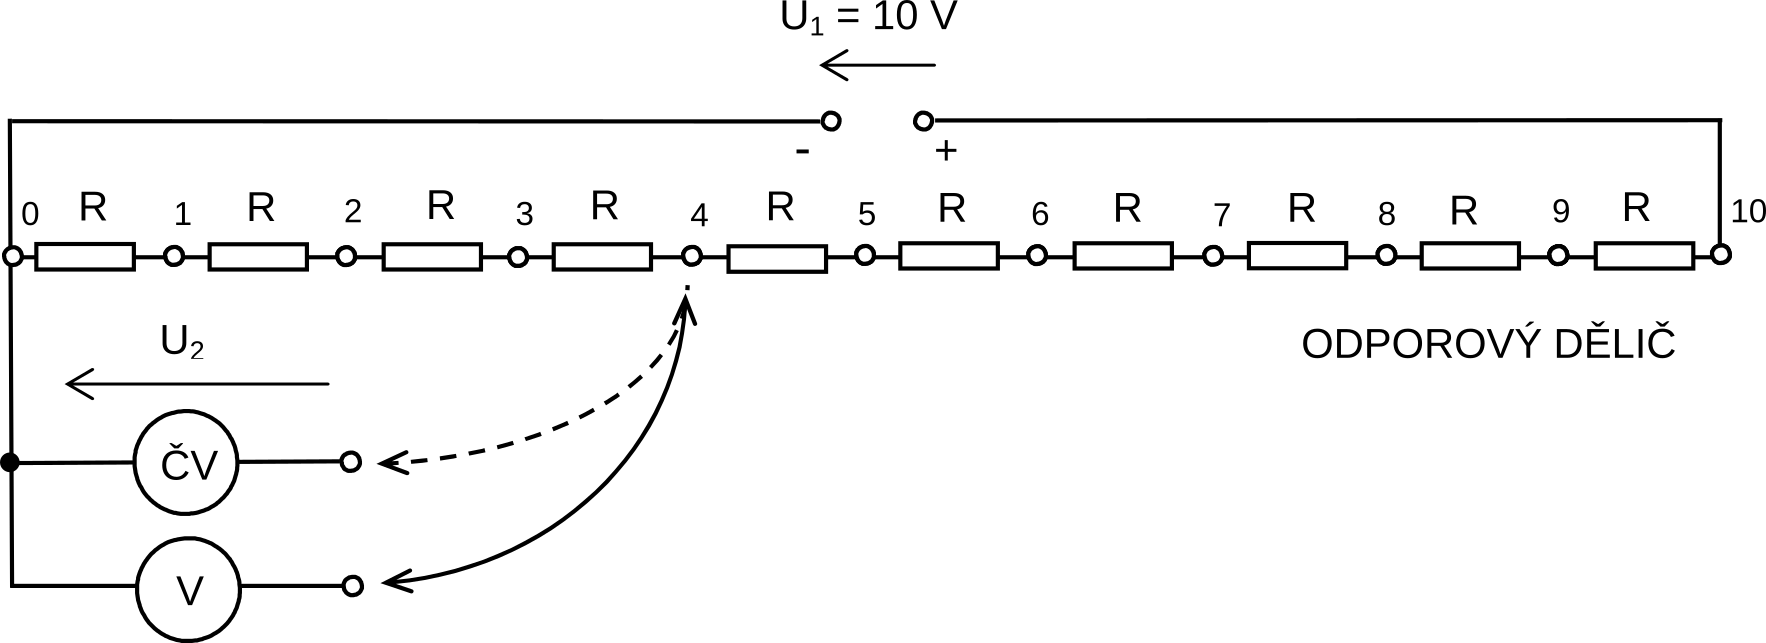
\includegraphics[scale=1.00]{LAB3.png}
\caption{Schéma zapojení}
\end{figure}
\section{Soupis použitých přístrojů}
\begin{tabular}{ll}
	V & voltmetr magnetoelektrický, tř.přes. $0.5$, rozsah $12 V$, odpor $500 \Omega/V$\\
	ČV & voltmetr číslicový, typ M1T 330, přesnost $\pm 0,01\%$ údaje $\pm 0,01\%$ rozsahu\\
	U1 & zdroj stejnosměrného napětí, typ AGILENT E3640A\\
	Př1 & odporový dělič
\end{tabular}

\section{Teoretický základ}

Pokud měříme odporový dělič voltmetrem se srovnatelným vstupním odporem s výstupním odporem děliče, je hodnota $U_2$ menší než hodnota na prázdno $U_0$ (Obr 2a). Skutečný dělič napájený napětím $U_0$ zatížený voltmetrem se vstupním odporem $R_V$ (Obr 2b) lye nahradit Theveninovým náhradním obvodem (Obr 2c). Poté pro $U_2$ platí:
\begin{equation}
U_2 = U_0 {R_v \over R_V + R_D}
\end{equation}
kde $R_D$ je výstupní odpor děliče.

\begin{figure}[h]
	\centering
	\begin{subfigure}{0.4\textwidth}
		\begin{circuitikz}[european]
			\draw (1,-0.0) to[R,l_=$R_2$] (1,-2.0);
			\draw (1,-0.0) to[R,l=$R_1$] (1,2.0);
			\draw (1,2.0) to[short] (0,2.0);
			\draw (0,-1.0) to[short] (0,-2.0);
			\draw (0,-2.0) to[short] (1,-2.0);
			\draw (0,-1.0) to[esource,l=$U_1$] (0,1.0);
			\draw (0,1.0) to[short] (0,2.0);
			\draw (1,-0.0) to[short] (2,-0.0);
			\draw (1,-2.0) to[short] (2,-2.0);
			\draw (2, 0) to[open, v^>=$U_0$] (2,-2);
		\end{circuitikz}
		\caption{naprázdno}
	\end{subfigure}
	\begin{subfigure}{0.4\textwidth}
		\begin{circuitikz}[european]
			\draw (0,-1.0) to[esource,l=$U_1$] (0,1.0);
			\draw (1,2.0) to[R,l_=$R_1$] (1,-0.0);
			\draw (1,-0.0) to[R,l_=$R_2$] (1,-2.0);
			\draw (1,-2.0) to[short] (0,-2.0);
			\draw (0,-1.0) to[short] (0,-2.0);
			\draw (1,2.0) to[short] (0,2.0);
			\draw (0,2.0) to[short] (0,1.0);
			\draw (1,-0.0) to[short] (2,-0.0);
			\draw (1,-2.0) to[short] (2,-2.0);
			\draw (2,0.0) to[rmeter, t=V, v^>=$U_2$] (2,-2.0);
		\end{circuitikz}
		\caption{zatížený voltmetrem (odpor $R_V$)}
	\end{subfigure}
	\begin{subfigure}{0.4\textwidth}
		\begin{circuitikz}[european]
			\draw (0,1.0) to[R,l=$R_D$] (2,1.0);
			\draw (0,-1.0) to[esource,l=$U_1$] (0,1.0);
			\draw (2,1.0) to[rmeter, t=V, v^>=$U_2$] (2,-1.0);
			\draw (2,-1.0) to[short] (0,-1.0);
		\end{circuitikz}
		\caption{nahrádní Théveninův obvod}
	\end{subfigure}
	\caption{Odporový dělič}
\end{figure} 

Připojením voltmetru vzniká chypa, pro níž platí
\begin{equation}
\Delta U_{met}=U_2-U_0=U_0{R_V \over R_V+R_D} - U_0 = U_0 {-R_D \over R_V + R_D }
\end{equation}

Má-li voltmetr vstupní odpor mnohem vyšší, než je odpor děliče, pak je chyba metody zanedbatelná. Pro číslicový voltmetr se vstupním odporem $R_{CV}  \approx  10^9 \Omega$ tedy naměříme $U_0 \cong U_{2CV}$.

Velikost výstupního odporu děliče můžeme zjistit buď z náhradního schématu 2c a vztahu (1),z něhož lze vyjádřit $R_D$:
\begin{equation}
R_D={R_V(U_{2CV}-U_2) \over U_2} = R_V({U_{2CV} \over U_2}-1)
\end{equation}
Nebo pomocí proudu odporem $R_D$:
\begin{equation}
R_D=|{U_{2CV}-U_2 \over -I_2}| = R_V({U_{2CV} \over U_2}-1)
\end{equation}
\subsection{Určení nejistoty měření výstupního odporu}

Pokud jsou fluktuace měření zanedbatelné vůči přesnosti přístroje udávané výrobcem, je nejistota typu A zanedbatelná a napětí $U_{2CV}$ a $U_2$ potřebná pro výpočet odporu $R_D$ je třeba změřit pouze jednou. Jinak je třeba měření několikrát opakovat a z jejich aritemtických průměrů dostat nejistoty typu A.\\
Lze přepokládat, že nejisoty typu A budou zanedbatelné a pro nejistotu $R_D$ tedy platí:
\begin{equation}
u_{RD}=\sqrt{({\partial R_D \over \partial U_{2CV}}u_{U2CV})^2+({\partial R_D \over \partial U_{2}}u_{U2})^2+({\partial R_D \over \partial R_{V}}u_{RV})^2}
\end{equation}
\end{document}
